\chapter*{Industrial Recognition: A Granted Patent}
\addcontentsline{toc}{chapter}{Industrial Recognition: A Granted Patent}
\markboth{Industrial Recognition: A Granted Patent}{Industrial Recognition: A Granted Patent}
\label{chap:patent}

% This chapter is unnumbered, so give its floats their own prefix instead of
% inheriting Chapter 5's counters.
\setcounter{figure}{0}
\renewcommand{\thefigure}{P.\arabic{figure}}
\setcounter{table}{0}
\renewcommand{\thetable}{P.\arabic{table}}

The industrial significance of the platform on which this internship was carried
out was formally recognized while the work was under way. The core Power-to-X
optimization method at the heart of the Energy Transition Optimizer is protected
by a United States patent granted to Boston Consulting Group,
\textbf{US~12,711,433~B2}, \emph{Systems and Techniques for Optimizing the
Implementation and Operation of Power-to-X Plants}, issued on 18~August~2026
\cite{bcgptx2026}. The application was filed in September~2023 and published in
March~2025, so the engine that this report treats as the numerical authority was,
throughout the internship, a patent-pending industrial asset, and its grant
landed as this report was being finalized. Table~\ref{tab:patent} gathers its
bibliographic details, and Figure~\ref{fig:patent-firstpage} reproduces the
patent's front page.

\begin{figure}[H]
  \centering
  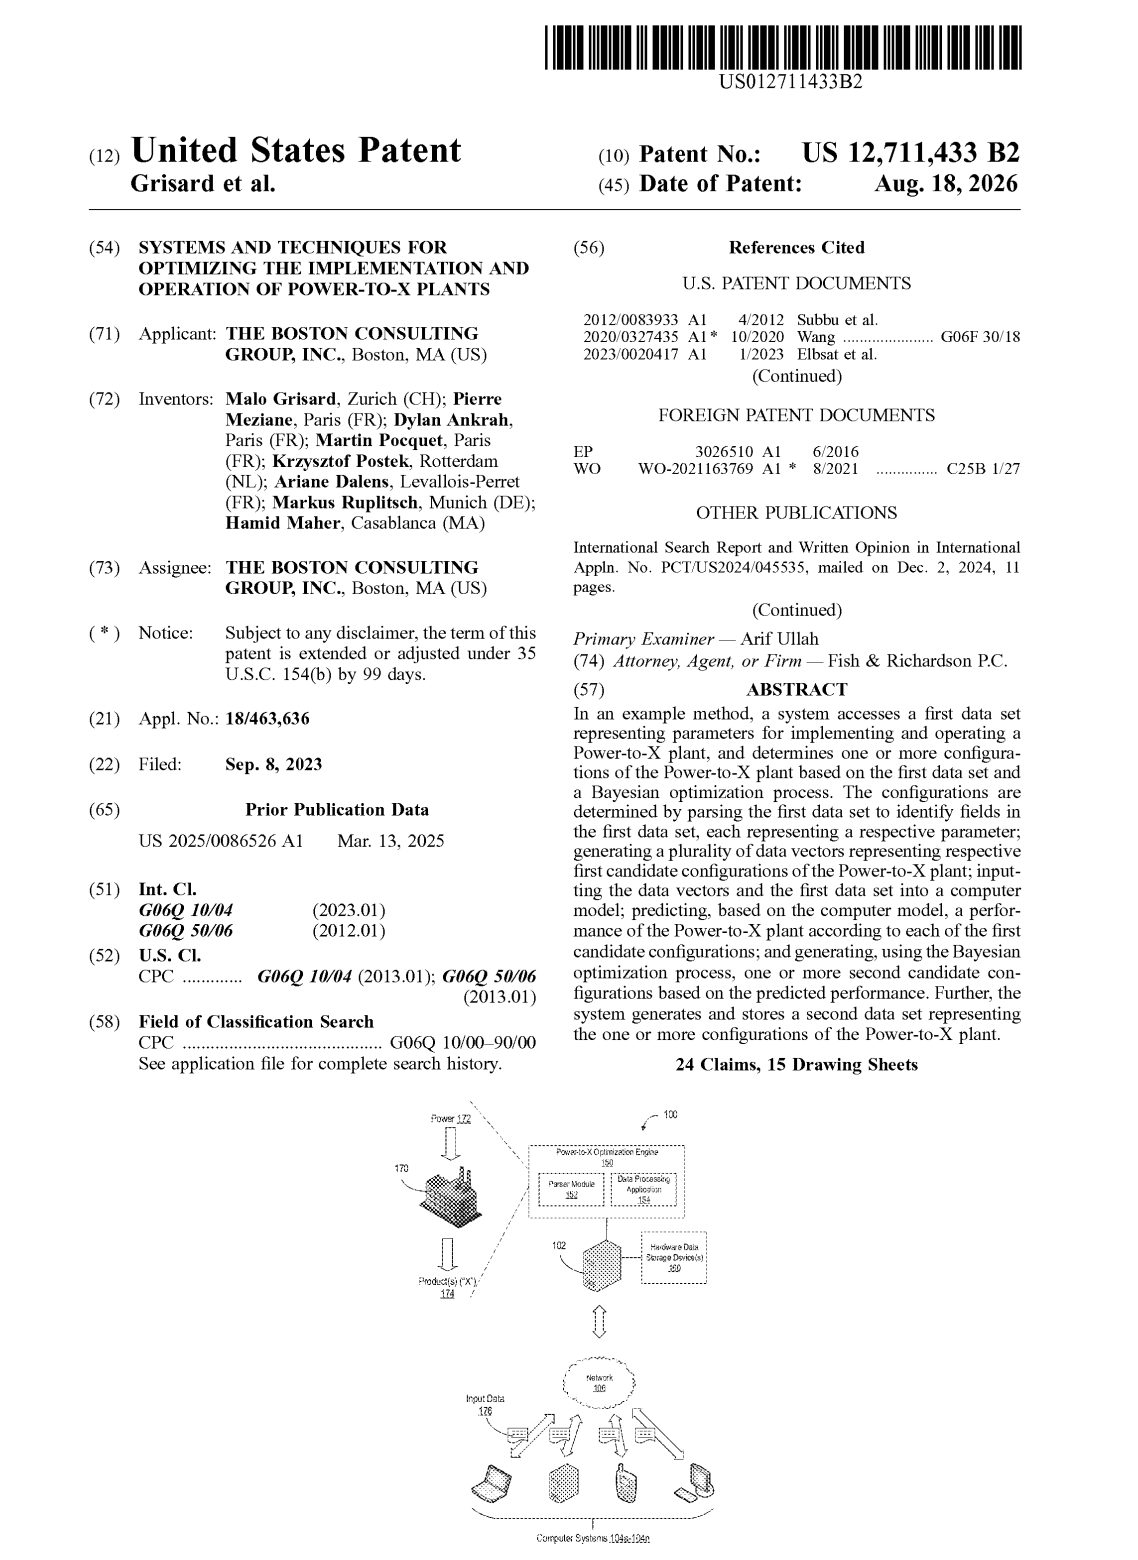
\includegraphics[width=0.8\linewidth]{Figures/patent.png}
  \caption{The granted patent US~12,711,433~B2: cover sheet of the public USPTO
    document.}
  \label{fig:patent-firstpage}
\end{figure}

\begin{table}[H]
  \centering
  \small
  \begin{tabularx}{\linewidth}{@{}>{\raggedright\arraybackslash}p{3.4cm} >{\raggedright\arraybackslash}X@{}}
    \toprule
    \textbf{Field} & \textbf{Detail} \\
    \midrule
    Patent number & US~12,711,433~B2 \\
    \addlinespace
    Title & Systems and Techniques for Optimizing the Implementation and
      Operation of Power-to-X Plants \\
    \addlinespace
    Assignee & The Boston Consulting Group, Inc. (Boston, MA, USA) \\
    \addlinespace
    Inventors & M.~Grisard, P.~Meziane, D.~Ankrah, M.~Pocquet, K.~Postek,
      A.~Dalens, M.~Ruplitsch, and H.~Maher \\
    \addlinespace
    Application & No.~18/463,636, filed 8~September~2023 \\
    \addlinespace
    Prior publication & US~2025/0086526~A1, 13~March~2025 \\
    \addlinespace
    Date of grant & 18~August~2026 \\
    \addlinespace
    Classification & G06Q~10/04; G06Q~50/06 (operations research and energy) \\
    \addlinespace
    Scope & 24~claims, 15~drawing sheets \\
    \bottomrule
  \end{tabularx}
  \caption{Bibliographic details of the granted patent covering the optimizer's
    core method.}
  \label{tab:patent}
\end{table}

\section*{What the patent protects}

The patent covers the optimizer's core method for determining strong plant
configurations. In the terms of its abstract, a system accesses a data set of
parameters for implementing and operating a Power-to-X plant, parses that data
set to identify the fields that represent each parameter, and generates a set of
data vectors that stand for candidate plant configurations. Those candidates and
the parameter set are passed to a computer model that predicts the performance of
the plant under each configuration, and a \textbf{Bayesian optimization} process
then proposes new candidate configurations from the predicted performance,
iterating toward strong designs and storing the resulting configurations.

This is the formal description of the capability that
Chapter~\ref{chap:context} introduced as the deterministic engine and its
parameter search: turning a typed description of a plant and its assumptions into
optimized, evaluated configurations with auditable financial indicators. The two
descriptions operate at different layers, and it is worth being precise about the
distinction. The patent's \textbf{Bayesian optimization} is a strategy for
\emph{choosing} which candidate configurations to evaluate next; each configuration
is then scored by the \textbf{deterministic} simulation that this report treats as
the numerical authority. The product as studied here drives that same deterministic
engine through an exhaustive \textbf{grid search} over the design space rather than
the patented Bayesian search, so the "deterministic engine and its parameter search"
of Chapter~\ref{chap:context} and the patented method share the deterministic
per-configuration evaluation while differing in how the design space is explored.

\section*{Relation to this work}

Two points connect this grant to the present report. First, it concerns the
\textbf{deterministic optimization core, not the governed agentic layer} that is
the subject of this internship. The application predates the internship, and the
author of this report is not among the named inventors; several members of the
team he worked with are, including the product's technical lead. The patent
therefore belongs to the surrounding product context established in
Chapter~\ref{chap:context}, not to the work detailed in
Chapters~\ref{chap:design} and~\ref{chap:implementation}. A granted patent
certifies novelty and industrial applicability in the legal sense; it is presented
here as industrial context, not as evidence of the system's performance or adoption,
which are the province of the evaluation in Chapter~\ref{chap:implementation}.

Second, and more importantly, the grant sharpens the central principle defended
throughout this report. The patented method is precisely the \emph{numerical
authority} that the agentic layer is designed to serve rather than replace: the
assistant prepares inputs, explains outputs, and guides the workflow, while the
protected optimization engine remains the sole source of the configurations and
the financial indicators. Building a governed, grounded assistance layer on top of
a patented core is exactly the product-level investment described in
Section~\ref{sec:internal-product}. It lowers the barrier to using a valuable,
protected capability for every future client adaptation, without diluting the
reproducibility and auditability that make that capability worth protecting. From
an industrial-property standpoint, the grant reinforces the same separation between
assistance and authority that this report upholds from an engineering one.
